\section{Referentni podaci}

Referentni podaci su oni podaci s kojima se uspoređuju rezultati metoda. Ti podaci su generirani u simulatoru te stanje vozila u jednome trenutku u vremenu. Referentni podaci se zapravo sastoje od lokacije i rotacije vozila.

\subsubsection{Lokacija}
Lokacija vozila je također definirana kao točka u kartezijevom koordinatnome prostoru. Sastoji se od x, y i z koordinata. Slično kao prikazano na slici \ref{fig:point_coordinates}.

\subsubsection{Rotacija}
 U trodimenzionalnome prostoru objekt se zapravo može rotirati oko beskonaćnoga broja osi ali se u pravilu uzimaju 3 statičke osi. Te osi se nazivaju os skretanja (eng. yaw), os poniranja (eng. pitch) i os valjanja (eng. roll). 

\begin{figure}[!ht]
  \centering
  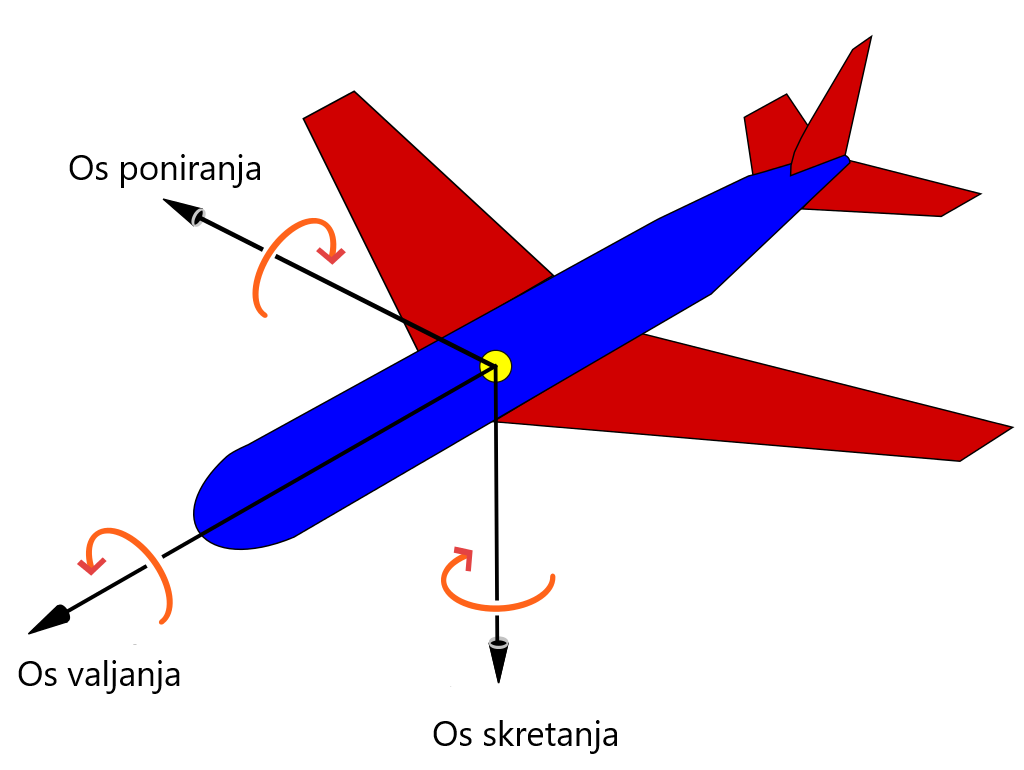
\includegraphics[scale=0.3]{images/yaw_roll_pitch_example.png}
  \caption{Ilustracija osi rotiranja \cite{apa}}
  \label{fig:yaw_roll_pitch_example}
\end{figure}

Os rotacije je os koja prolazi u smjeru kretanja vozila (x os), os poniranja je zapravo os okomita s os rotacija (z os), dok je os skretanja okomita na obje prethodne osi (y os). Te osi su ilustrirane na slici \ref{fig:yaw_roll_pitch_example}. Rotacija između dva sustava može biti reprezentirana pomoću rotacijskih matrica\cite{wiki:Rotation_matrix}. Te matrice su veličine 3x3 te predstavljaju rotaciju oko određene osi.
\pagebreak

\begin{equation}
  R_{x}(\alpha) =
  \begin{pmatrix}
    1 & 0 & 0\\
    0 & cos(\alpha) & -sin(\alpha)\\
    0 & sin(\alpha) & cos(\alpha)
  \end{pmatrix}
  \label{mat:rot_mat_x}
\end{equation}

\begin{equation}
  R_{y}(\beta) =
  \begin{pmatrix}
    cos(\beta) & 0 & sin(\beta)\\
    0 & 1 & 0\\
    -sin(\beta) & 0 & cos(\beta)
  \end{pmatrix}
  \label{mat:rot_mat_y}
\end{equation}

\begin{equation}
  R_{z}(\gamma) =
  \begin{pmatrix}
    cos(\gamma) & -sin(\gamma) & 0\\
    sin(\gamma) & cos(\gamma) & 0\\
    0 & 0 & 1
  \end{pmatrix}
  \label{mat:rot_mat_z}
\end{equation}

Za razliku od rotacijskih matrica Eulerova reprezentacija rotacije se sastoji od samo 3 broja. Ta tri broja opisuju sekvencu kojom je objekt rotiran. Rotacija se može opisati na 12 načina zato što se prikazuje dinamička rotacija. Primjeri su XYX, ZZX, ZYZ, itd. Objekt u trodimenzionalnome prostoru možemo rotirati pomoću matrica \ref{mat:rot_mat_x}, \ref{mat:rot_mat_y} i \ref{mat:rot_mat_z} u prethodni dogovor da se prvo rotira oko x osi, tada oko y osi i naposljetku oko z osi pomoću formule \ref{eq:rotate_point} gdje su $\alpha$, $\beta$ i $\gamma$ kutevi rotacije oko x, y i z osi.

\begin{gather}
    \begin{bmatrix} X_{t}\\ Y_{t}\\ Z_{t} \end{bmatrix}
    =
    R(\gamma)R(\beta)R(\alpha)
    \begin{bmatrix} X_{o}\\ Y_{o}\\ Z_{o} \end{bmatrix}
    \label{eq:rotate_point}
\end{gather}
Kao kompromis između prednosti i nedostataka prethodnih reprezentacija rotacije objekata koristi se sustav kvaterniona\cite{wiki:Quaternion} (eng. Quaternion). U matematici kvaterniona su skup brojeva koji proširuju kompleksne brojeve. Rotacija je prikazana kao vektor od 4 komponente. Formula \ref{eq:quat_multiply} prikazuje kako se množe kvaternioni.

\begin{equation}
  i^2 = j^2 = k^2 = ijk = -1
  \label{eq:quat_multiply}
\end{equation}
Jedan kvaternion (jedinični) je definiran kao zbroj skalara $a$ i vektora $[a b c]$ te iznosi:

\begin{equation}
  q = a + b\hat{i} + c\hat{j} + d\hat{k}
  \label{eq:jedinicni_vektor}
\end{equation}
Ako os rotacije napišemo u obliku $u=u_{x}\hat{i} + u_{y}\hat{j} + u_{z}\hat{k}$ gdje su $u_{x}$, $u_{y}$ i $u_{z}$ kalarne veličine te je $\theta$ kut zakreta te iste osi tada se rotacija može zapisati kao:

\begin{equation}
  q=\cos(\frac{\theta}{2})-(u_{x}i + u_{y}j + u_{z}k)\sin(\frac{\theta}{2})
\end{equation}
Pretvorba kvaterniona u generalnu rotacijsku matricu se provodu na sljedeći način:

\begin{equation}
R = 
  \begin{pmatrix}
    a^2 + b^2 - c^2 - d^2 & 2bc - 2ad & 2bd + 2ac \\
    2bc + 2ad & a^2 - b^2 + c^2 - d^2 & 2cd - 2ab \\
    2bd - 2ac & 2cd + 2ab & a^2 + b^2 - c^2 + d^2
  \end{pmatrix}
  \label{eq:qvat_to_rot_mat}
\end{equation}